\setcounter{page}{1}
\section*{Zielsetzung}
In dem Versuch $V64$ wird mittels eines \emph{Sagnac Interferometers}
der Brechungsindex $n$ von Luft und einer Glasplatte bestimmt.
Hierbei bietet ein Sagnac Interferometer den Vorteil, einer
besseren Stabilität gegenüber externen Störung, als zum Beispiel
ein Michelson Interferometer. Geschuldet ist die höhere Stabilität
dem Fakt, dass die Lichtstrahlen des Interferometers den selben Weg zurücklegen.

\section{Theorie}
Der Brechungsindex $n$ wird mit einem Interferometer mit Hilfe von
Interferenzeffekten bestimmt. Interferenzen entstehen durch
eine Phasendifferenz $\Delta\phi$ zwischen zwei kohärenten Lichtstrahlen.
Eine solche Phasendifferenz wird in Gasen und Festkörpern unterschiedlich erzeugt.
Bevor auf diese Problemstellung eingeangen wird, werden zunächst Interferenzen
mit dem Wellencharakter von Licht motviert.
%Brechungsindex von Gasen
%Brechungsindex von Festkörpern(Glasen)
%Polarisation
\subsection{Beschreibung von Licht}
Licht kann als elektromagnetische Welle beschrieben werden.
Auf Grund der Kopplung des elektrischen und magnetischen Teiles reicht
es für eine vollständige Beschreibung von Licht aus, nur einen der beiden Teile zu untersuchen.
Im Folgenden betrachten wir deshalb den elektrischen Teil.
Für monochromatisches Licht kann das elektrische Feld $\vec{E}$ mathematisch beschrieben
werden durch
\begin{equation*}
  \vec{E} = \vec{E_0} \map{exp}\left(i (\omega t-\vec{k}\vec{r})\right),
\end{equation*}
hierbei repräsentiert $\vec{E_0}$ die Polarisation des Feldes.
Die Überlagerung von zwei Wellen $\vec{E}_1$ und $\vec{E}_2$ kann zu Interferenzeffekten führen.
Im allgemeinen gilt dabei für die Intensität der überlagerten Wellen:
\begin{align}
  \label{eq:Interferenz_enstehung}
  \begin{aligned}
  \vec{E}_1&=\vec{E}_{0,1} \map{exp}\left(i (\omega t-\vec{k}\vec{r})\right), \qquad \vec{E}_2 =\vec{E}_{0,2} \map{exp}\left(i (\omega t-\vec{k}\vec{r}+\Delta\phi)\right) \\
  I &\propto \left<\be{E_1+E_2}^2\right> = E_{0,1}^2 + E_{0,2}^2 + 2E_{0,1}E_{0,2}\cos(\delta)\cos(\Delta\phi),
\end{aligned}
\end{align}
wobei $\Delta\phi$ die Phasendifferenz zwischen $\vec{E_1}$ und $\vec{E_2}$ darstellt und
$\delta$ den Polarisationswinkel der beiden Feldervektoren repräsentiert.
Die Art der Interferenz hängt somit von der Phasendifferenz ab:
\begin{align}
  \Delta\phi &=0,2\pi,4\pi,\dots \qquad \text{Konstruktive Interferenz} \label{eq:Konstruktive}\\
  \Delta\phi &= \pi, 3\pi, 5\pi,\dots \qquad \text{Destruktive Interferenz}. \label{eq:Destruktive}
\end{align}
Anzumerken ist, dass senkrecht zueinander polarisiertes Licht $\delta=\frac{\pi}{2}$ nicht
interferenzfähig ist.
\subsection{Brechungsindex von Gasen}
Propagiert ein Lichtstrahl von Medium $A$ durch eine Gasezelle der Länge $L$ mit Medium $B$,
so führt das zu einer Phasendifferenz $\Delta\phi$ relativ gesehen zu einem Lichtstrahl, der sich
nur durch Medium $A$ bewegt. Erzeugt wird diese Phasendifferenz durch die Änderung der
Phasengeschwindigkeit im Medium $v\ua{ph}=\frac{\map{c}}{n_B}=\frac{\omega}{k}$, wobei $\map{c}$
die Vakuumlichtgeschwindigkeit darstellt. Eine Änderung der Phasengeschwindigkeit
verursacht eine Änderung der Wellenzahl $k$ und somit eine Phasenverschiebung
\begin{equation}
  \label{eq:phase_shit_gases}
\Delta\phi = kL = \frac{2\pi}{\lambda\ua{vac}}(n_B-n_A)L,
\end{equation}
mit der Vakuumwellenlänge $\lambda\ua{vac}$ und den Brechungsindizeis der
Medien $A$ und $B$.
Zu beachten ist, dass der Brechungsindex eines Gases allgemein von dem Druck $p$ abhängt.
Beschrieben wird diese Druckabhängigkeit durch das Lorentz-Lorenz Gesetz.
Im Rahmen dieses Protokolls wird eine genährte Variante des Gesetzes verwendet,
welches der Quelle \cite{lorentz} entnommen ist:
\begin{equation}
  \label{eq:lorentz}
  n\approx \sqrt{1+\frac{ 3Ap }{ \map{R}T } }.
\end{equation}
Die in Gleichung \eqref{eq:lorentz} auftretenden Größen sind
zum einen die Gaskonstante $\map{R}$, die Temperatur $T$ und der
molare Brechungsindex $A$.
Die Druckabhängigkeit wird in einem Interferometer verwendet, um zwei kohärente Strahlen interferieren zu lassen.
Durch eine Beobachtung bzw. Zählung der Interferenzmaxima $M$, bei einer gegebenen Druckdifferenz, ist es möglich den Brechungsindex zu bestimmen.
Hierbei gilt für die Anzahl der Maxima bei einem gegebenen Druck der folgende Zusammenhang:
\begin{equation}
  \label{eq:anzahl_maxima_gas}
  M=\frac{\Delta\phi}{2\pi}= \frac{ n_B-n_A }{ \lambda\ua{vac} }L.
\end{equation}
\subsection{Brechungsindex von Festkörpern}
Im Gegensatz zu Gasen hängt Brechungsindex eines Festkörpers kaum vom Druck ab.
Deshalb muss hier eine andere Methodik zur Ermittlung des Brechungsindexes verwendet werden.
Propagiert ein Lichtstrahl, wie in Abbildung \ref{fig:slag} gezeigt, durch einen Festkörper der Länge $T$,
so wird dieser nach dem Snelliussches Brechungsgesetz gebrochen.
\begin{figure}
\centering
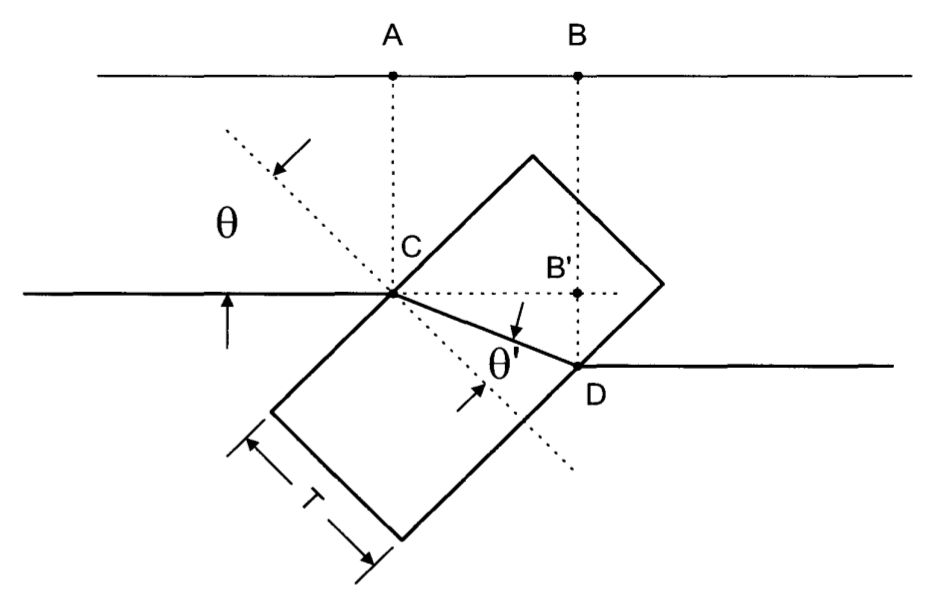
\includegraphics[width=0.6\linewidth]{./content/images/slab.png}
\caption{Ein Lichtstahl propagiert durch einen Festkörper z.\,B. Glas der Länge $T$ \cite{anleitung64}.}
\label{fig:slag}
\end{figure}
Hierdurch entsteht ein Gangunterschied, der sich in eine Phasendifferenz übersetzt.
Mathematisch bestimmt werden kann die Phasendifferenz über den folgenden Zusammenhang
\begin{equation}
  \label{eq:Phasendifferenz_festkörper}
  \Delta\phi=\frac{ 2\pi T }{ \lambda\ua{vac} }\left( \frac{ n-\cos(\theta-\theta') }{ \cos(\theta') } - n+1\right),
\end{equation}
wobei $n$ der Brechungsindex des Festkörpers repräsentiert.
Mit Hilfe einer Kleinwinkelnäherung von $\theta$ und dem Snelliussches Brechungsgesetz kann
Gleichung \eqref{eq:Phasendifferenz_festkörper} vereinfacht werden zu:
\begin{equation}
  \Delta\phi=\frac{ 2\pi T }{ \lambda\ua{vac} }\left( \frac{ n-1 }{ 2n }\theta^2 + \mathcal{O}(\theta^4)\right)
\end{equation}
Mit der Phasendifferenz ist es nun möglich die Anzahl an Interferenzmaxima $M$ anzugeben, die bei einer Drehung
des Festkörpers um den Winkel $\theta$ entstehen. Zu beachten ist, dass der Laserstrahl, in einem Interferometer, zweimal den Festkörper durchquert
\begin{equation}
  \label{eq:Interferenzmaxima_solid_state}
  M=2\frac{\Delta\phi}{2\pi}\approx \frac{T}{\lambda\ua{vac}}\frac{n-1}{2n}\theta^2.
\end{equation}
Die Gleichung \eqref{eq:Interferenzmaxima_solid_state} wird im folegenden
durch den linearen Term einer Taylorentwicklung umgeschrieben:
\begin{equation}
\label{eq:entwicklung_interferenzmaxima}
  M\approx\frac{T}{\lambda\ua{vac}}\frac{n-1}{n}\left( 2\theta(\theta-\theta_0)\right).
\end{equation}
\subsection{Polarisation}
Bisher wurde lediglich der Wellencharakter von Licht betrachtet. Jedoch besitzt eine
elektromagnetische Welle einen weiteren Freiheitsgrad, die Polarisation.
Die Polarisation gibt die Richtung des elektrischen Feldvektors an.
Eine Änderung der Polarisation kann mit Hilfe von Polarisationsfiltern bewirkt werden.
Der Filter absorbiert den Lichtanteil, welcher um $\frac{\pi}{2}$ zum eingestellt Filterwinkel
gedreht ist. Somit wird die Polarisation des transmittierte Lichtes auf die Filterachse projiziert (vgl. Abb. \ref{fig:pola}).
\begin{figure}
\centering
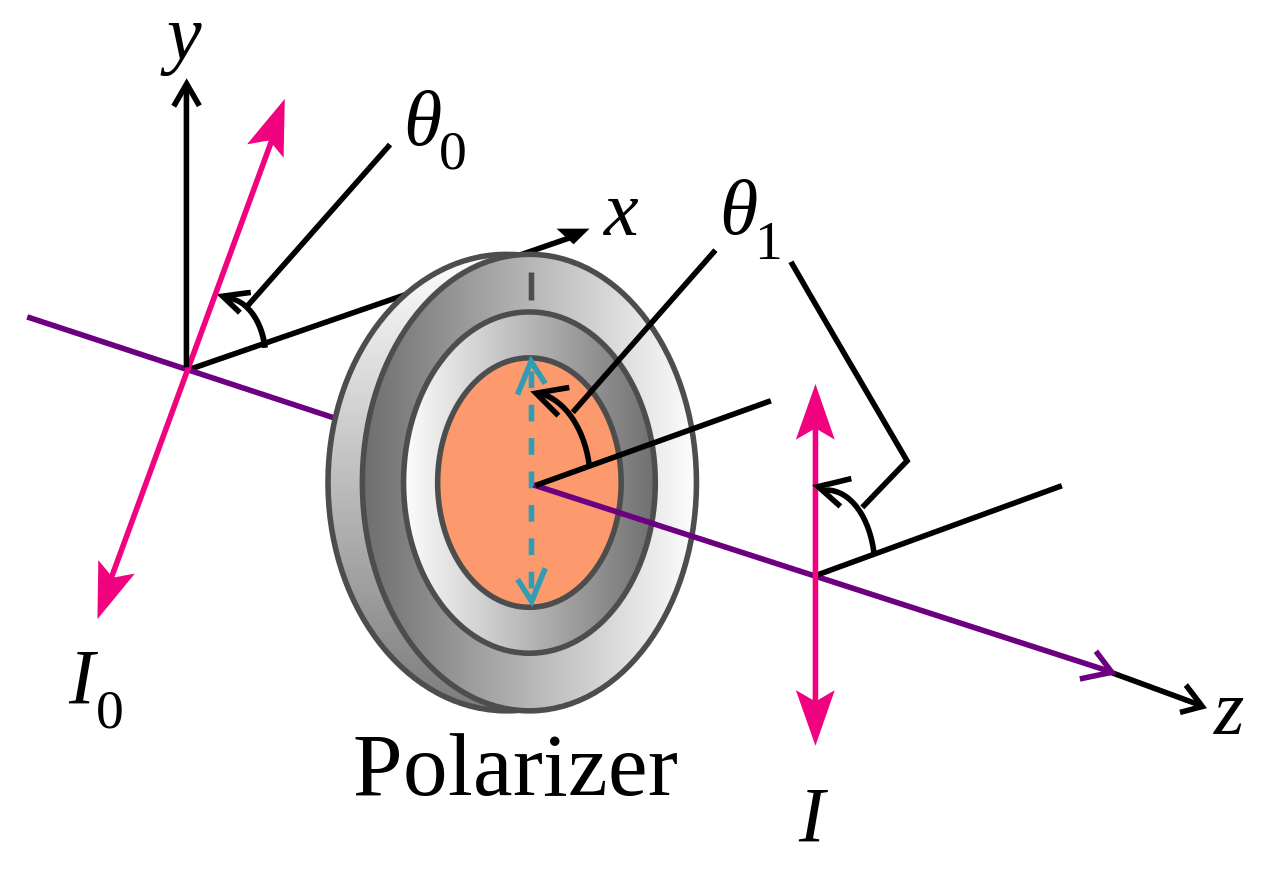
\includegraphics[width=0.5\linewidth]{./content/images/polarisationsfilter.png}
\caption{Schematische Darstellung der Polarisationsänderung durch ein Polarisationsfilter \cite{pola}.}
\label{fig:pola}
\end{figure}

Zusätzlich werden in dem Versuch \emph{polarizing beam-splitter cubes} (PBSCs) verwendet.
Hergestellt wird ein solcher Würfel, wenn zwei $45-45-\SI{90}{\degree}$ Prismen
an der Hypotenuse mit einander verklebt werden. Wichtig ist das auf dieser, vor dem verkleben,
eine dielektrische Schicht aufgebracht wird. Ein PBSC teilt den auftreffenden Strahl
in zwei Strahlen auf, die orthogonal in Ausbreitungsrichtung und Polarisation
sind (vgl. Abb. \ref{fig:pbsc}).
\begin{figure}
\centering
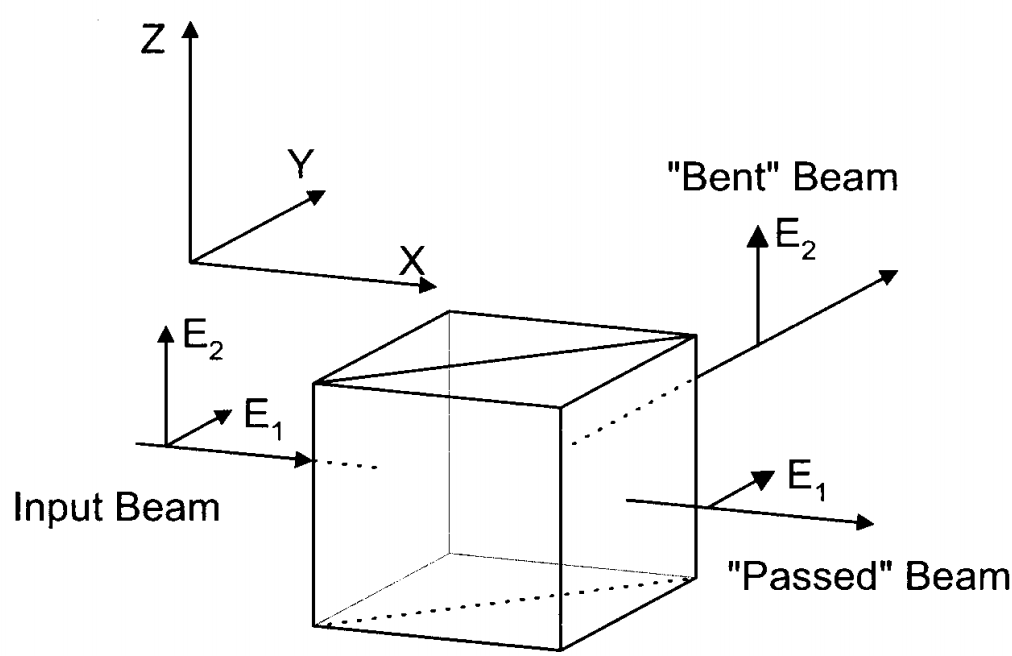
\includegraphics[width=0.6\linewidth]{./content/images/pbsc.png}
\caption{Schematische Darstellung eines PCBS \cite{anleitung64}.}
\label{fig:pbsc}
\end{figure}
